\chapter{Symmetry Energy}
\label{ap:symmetry_energy}
$$ E_k = C(N^{5/3} + Z^{5/3}) $$
Let: $A = N + Z$ and $B = N - Z$, then we have $N + \frac{A+B}{2}$, 
$Z = \frac{A-B}{2}$ and $B << A$:
\begin{equation*}
    \begin{aligned}
	E_k &= C\left( \left( \frac{A+B}{2}\right)^{5/3} + \left(\frac{A-B}{2} \right)^{5/3} \right)	\\
	    &= C\left(\frac{A}{2}\right)^{5/3} \left( \left( 1 + \frac{B}{A} \right)^{5/3} + \left(1 - \frac{B}{A} \right)^{5/3} \right)   \\
	    &= C\left(\frac{A}{2}\right)^{5/3} \left( \left(1 + \frac{5}{3}\frac{B}{A} + \frac{1}{2!}\frac{5}{3}\frac{2}{3} \left( \frac{B}{A} \right)^2 + \cdots \right) 
		+ \left(1 + \frac{5}{3}\left(-\frac{B}{A} \right) + \frac{1}{2!}\frac{5}{3}\frac{2}{3} \left( -\frac{B}{A} \right)^2 + \cdots \right) \right) \\
	    &= 2^{-2/3}C\left( A^{5/3} + \frac{5}{9}\frac{B^2}{A^{1/3}} \right) + O(\frac{B^4}{A^{7/3}})	\\
	    &= 2^{-2/3}C\left( A^{5/3} + \frac{5}{9}\frac{(N-Z)^2}{A^{1/3}} \right) + O((N-Z)^4)	\\
    \end{aligned}
\end{equation*}

\begin{figure}
    \centering
    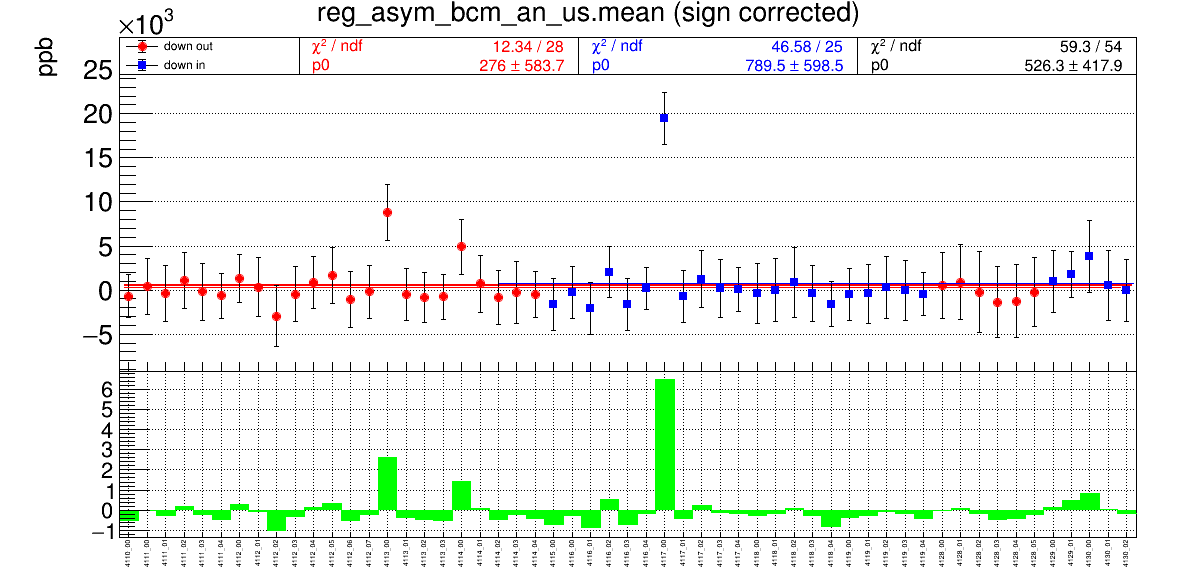
\includegraphics[width=\linewidth]{at/mini_prex_Pb_reg_asym_bcm_an_us.mean.png}
    \caption{charge asymmetry outlier in run 4117, minirun 0}
\end{figure}

\section{\Pb Foils Measurement}
\begin{landscape}
\begin{table}
    \centering
    \begin{tabular}{c | c | c c c c c c c c | c c c}
	\hline
	\multirow{2}{*}{Pb \#}	& \multirow{2}{*}{\thead{mass \\ (g)}}   & \multicolumn{2}{c}{\thead{top left\\ (mm)}}   & \multicolumn{2}{c}{\thead{top right\\ (mm)}}   & \multicolumn{2}{c}{\thead{bottom right\\ (mm)}}   & \multicolumn{2}{c|}{\thead{bottom left\\ (mm)}}   & \multirow{2}{*}{\thead{area \\ ($mm^2$)}} & \multirow{2}{*}{\thead{t \\ ($\mu m$)}}   & \multirow{2}{*}{\thead{area density \\ ($mg/cm^2$)}}	\\
	\cline{3-10}
	    &	& x1	& y1	& x2	& y2	& x3	& y3	& x4	& y4	&   &	&   \\
	\hline
	1   & 3.6526	& 0.005	    & -0.015	& 24.221    & 0.532	& 24.956    & -23.743	& 0.655	    & -24.249	& 588.3778  & 545.51	& 620.792	\\
	2   & 3.6973	& -0.005    & -0.012	& 24.079    & -0.2	& 23.897    & -24.338	& -0.327    & -24.294	& 584.7683  & 555.60	& 632.267	\\
	3   & 3.6325	& -0.009    & 0.01	& 24.156    & -0.039	& 24.08	    & -24.06	& -0.194    & -23.904	& 580.4809  & 549.89	& 625.774	\\
	4   & 3.6722	& -0.013    & -0.003	& 24.1	    & -0.302	& 24.048    & -24.386	& -0.133    & -24.363	& 584.8886  & 551.71	& 627.846	\\
	5   & 3.6989	& -0.002    & -0.001	& 24.199    & 0.003	& 24.261    & -24.136	& 0.083	    & -24.249	& 585.2287  & 555.40	& 632.044	\\
	6   & 3.6162	& -0.005    & -0.001	& 24.328    & -0.223    & 24.012    & -24.386	& 0.026	    & -24.276	& 585.1189  & 543.08	& 618.028	\\
	7   & 3.6966	& 0.001	    & 0.003	& 24.208    & 0.007	& 24.155    & -23.991	& 0.022	    & -23.869	& 578.5090  & 561.50	& 638.988	\\
	8   & 3.6315	& 0.008	    & 0.002	& 24.115    & 0.016	& 23.969    & -24.312	& -0.158    & -24.204	& 585.2472  & 545.26	& 620.507	\\
	9   & 3.6307	& 0.005	    & 0.003	& 24.216    & -0.268    & 23.992    & -24.704	& -0.149    & -24.421	& 590.6197  & 540.18	& 614.727	\\
	10  & 3.6283	& -0.052    & -0.029	& 23.973    & -0.225	& 24.032    & -24.234	& -0.297    & -24.213	& 582.5811  & 547.27	& 622.797	\\
	\hline
    \end{tabular}
    \caption{area was calculated as $A = \frac{(x2 - x1) + (x3 - x4)}{2} \times \frac{(y1 - y3) + (y2 - y4)}{2}$. 
    \Pb density is $11.38\ g/cm^2$.}
\end{table}
\end{landscape}

\begin{table}
    \centering
    \begin{tabular}{c c | c c c | c c c}
	\hline
	\multirow{2}{*}{run} & \multirow{2}{*}{\#entry}	& \multicolumn{3}{c|}{$\theta$}	& \multicolumn{3}{c}{$Q^2$} \\
	\cline{3-8}
	    &	& mean & RMS	& mean error	& mean	& RMS	& mean error	\\
	\hline
	1853	& 248697    & 4.741 & 0.447	& 8.96E-4    & 0.006239    & 0.001204    & 2.41E-6    \\
	1983	& 746777    & 4.747 & 0.4536	& 5.25E-4    & 0.006264    & 0.001223    & 1.42E-6    \\
	1996	& 513128    & 4.740 & 0.4461	& 6.23E-4    & 0.006244    & 0.001203    & 1.68E-6    \\
	2052	& 573912    & 4.741 & 0.444	& 5.86E-4    & 0.006246    & 0.001198    & 1.58E-6    \\
	2199	& 387046    & 4.751 & 0.466	& 7.49E-4    & 0.006286    & 0.001259    & 2.02E-6    \\
	2291	& 250751    & 4.753 & 0.4633	& 9.25E-4    & 0.006282    & 0.001248    & 2.49E-6    \\
	2292	& 188412    & 4.753 & 0.4622	& 1.06E-3    & 0.006281    & 0.001244    & 2.87E-6    \\
	2293	& 248789    & 4.754 & 0.4637	& 9.30E-4    & 0.006284    & 0.001249    & 2.50E-6    \\
	2294	& 190029    & 4.752 & 0.462	& 1.06E-3    & 0.00628	   & 0.001244    & 2.85E-6    \\
	2316	& 21379	    & 4.752 & 0.464	& 3.17E-3    & 0.00628	   & 0.001252    & 8.56E-6    \\
	2317	& 105672    & 4.746 & 0.4634	& 1.43E-3    & 0.006266    & 0.001251    & 3.85E-6    \\
	2319	& 15100	    & 4.746 & 0.4621	& 3.76E-3    & 0.006266    & 0.001247    & 1.01E-5    \\
	2320	& 100386    & 4.742 & 0.4607	& 1.45E-3    & 0.006254    & 0.001243    & 3.92E-6    \\
	\hline
	20981	& 245995    & 4.808 & 0.4409	& 8.89E-4    & 0.006401    & 0.001202    & 2.42E-6    \\
	21415	& 156514    & 4.814 & 0.4576	& 1.16E-3    & 0.006427    & 0.001245    & 3.15E-6    \\
	21435	& 19780	    & 4.816 & 0.4597	& 3.27E-3    & 0.006434    & 0.001256    & 8.93E-6    \\
	21436	& 367261    & 4.812 & 0.4585	& 7.57E-4    & 0.006424    & 0.001252    & 2.07E-6    \\
	21438	& 59044	    & 4.814 & 0.461	& 1.90E-3    & 0.006428    & 0.001259    & 5.18E-6    \\
	\hline
    \end{tabular}
    \caption{Optics data. The database used here was different from the final version.
    That's why the scattering angles were different from that in the published paper.}
\end{table}
\begin{comment}
\section{Resource}
\begin{itemize}
    \item hall A equipment: https://hallaweb.jlab.org/equipment/
\end{itemize}
\end{comment}
